\documentclass{standalone}
\author{Quinten Bruynseraede}
\usepackage{tikz}
\usetikzlibrary{shapes}
\title{Tikz grafen}
\begin{document}\pagestyle{empty}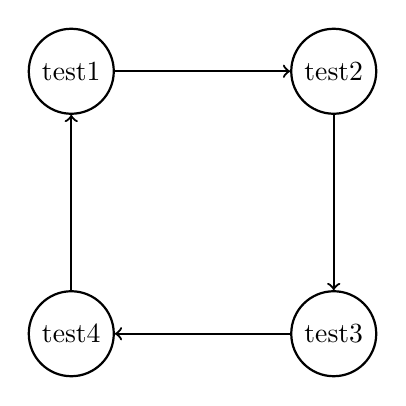
\begin{tikzpicture}\node[shape=circle,draw=black,align=center,line width=0.8pt] (0) at (3.3333333333333335,12.5) {test1};
\node[shape=circle,draw=black,align=center,line width=0.8pt] (1) at (6.666666666666667,12.5) {test2};
\node[shape=circle,draw=black,align=center,line width=0.8pt] (2) at (6.666666666666667,9.166666666666666) {test3};
\node[shape=circle,draw=black,align=center,line width=0.8pt] (3) at (3.3333333333333335,9.166666666666666) {test4};

\path [->,draw=black,line width=0.8pt] (0) edge node {} (1);
\path [->,draw=black,line width=0.8pt] (1) edge node {} (2);
\path [->,draw=black,line width=0.8pt] (2) edge node {} (3);
\path [->,draw=black,line width=0.8pt] (3) edge node {} (0);
\end{tikzpicture}
\end{document}